\chapter{Solution}
\label{ch:Solution}
This chapter presents the solution to tackle the issue of microservice identification. 
As noted in the \textit{State of the Art} chapter \ref{ch:StateOfTheArt}, existing approaches support two initial situations: They either conduct the extraction of microservices from existing (monolithic) systems or they are based on microservice greenfield development. Both types have their advantages and disadvantages. Existing systems, for instance, provide more information about the system specification and requirements. Legacy code and log files can be used to extract data dependencies or process structures. However, shortcoming in the design of the legacy application might have an impact on the extracted information and influence the microservice extraction in a negative manner. In contrast, greenfield development is not affected by any previously committed design decisions. As a matter of fact, the greenfield approach can be applied to existing systems as well by discarding legacy code and additional information that arose during the development. Solely the system requirements that existed before the implementation started serve as input. Nevertheless, this type has to manage the identification process with less input.\\
The solution we propose is based on pre-existing system requirements. No existing implementation is used and consequently, the presented approach is to be classified as greenfield method.\\



\section{Basic Approach}


\vspace{0.5cm}
\par
\begingroup
\leftskip=1cm
\rightskip=1cm

\noindent
\textbf{RQ1: Which is the most appropriate strategy to decompose a system into microservices? }

\endgroup
\vspace{0.5cm}



\noindent
This thesis proposes a formal, graph-based microservice identification approach using clustering on control flow and data flow. It is  inspired by Amiri’s work on \textit{Object-aware Identification of Microservices} \cite{ObjectAwareAmiri}. In chapter \ref{ch:StateOfTheArt}, eight suitable approaches to identify microservices are presented and compared using well-defined criteria. Most of them require special prerequisites and cannot be applied to various types of systems, i.e. no greenfield applications, systems without meaningful VCS meta-data or the absence of log files.
\\
By the way of contrast, Amiri proposes an approach to extract structural and data object dependencies from business point of view in order to generate possible microservice candidates. In doing so, he relinquishes to use any further information besides BPMN models. Using both, structural and data object dependencies promotes high cohesiveness and loose coupling on functional and data object level. In other words, high cohesive functionality is divided into the same microservices, together with the data objects that are accessed. \\
However, Sec.\ref{sec:stateOfTheArt:comparison} outlines the limitations and drawbacks of the approach. Whereas the control flow is depicted clearly, the data flow remains vague. The weight definitions regarding data object dependencies lack formal explanation. Further, the aggregation of structural and data object dependencies, and consequently the aggregation of control flow and data flow contains a significant problem: In Amiri's approach, the aggregation is conducted by summing up two relation matrices. The matrix entries representing the dependencies highly influence the results. For instance, a large amount of data reads and writes sum up to great numbers, outweighing the structural dependencies. Thus, the identification process would be almost based on data dependencies only, discarding any identified structural dependencies. \\
The following sections introduces a formal approach to tackle \textit{RQ2}. First, a basic overview of the approach is provided. Afterwards, each step is introduced in detail including alternatives and examples. 




\vspace{0.5cm}
\par
\begingroup
\leftskip=1cm
\rightskip=1cm

\noindent
\textbf{RQ2: What formal approach can be constructed to identify possible microservices without detailed know-how and manual effort? }

\endgroup
\vspace{0.5cm}



\noindent
To that end, Fig.\ref{fig:thesisProcess} provides an overview of the proposed approach. As depicted previously, the process requires input in form of BPMN models. Therefore, specifying those models marks the beginning of the process. Afterwards, control flow and data flow need to be extracted. To avoid the ambiguity of aggregating data flow and control flow as proposed by Amiri, the approach recommends to create two independent weighted Graphs, using the information from the previous step. In the next step, a clustering algorithm determines two sets of clusters based on the weights in the graphs. At that point, the process determined a set of clusters that is based on the structural dependencies and another one, based on data object dependencies. In the following, a matching process identifies commonalities between data object-based and structural-based clusters in order to create comprehensive clusters. Based on these clusters, the last step extracts microservice candidates. \\
%TODO  stimmt das noch?
\textit{RQ2} also broaches the subject of necessary know-how and the amount of manual effort. As far as that is concerned, the proposed approach does not require human interaction as soon as the BPMN models are specified. Everything beyond that is based on a structural process.
Admittedly, the manual effort to conduct the process entirely is still not to be neglected, as the extraction process, graph creation and cluster matching is not yet automated. Nevertheless, the structural process enables to implement the entire approach, excluding the BPMN model specification step. However, implementing an approach is beyond the scope of the paper.




 
\begin{figure}[h!]
	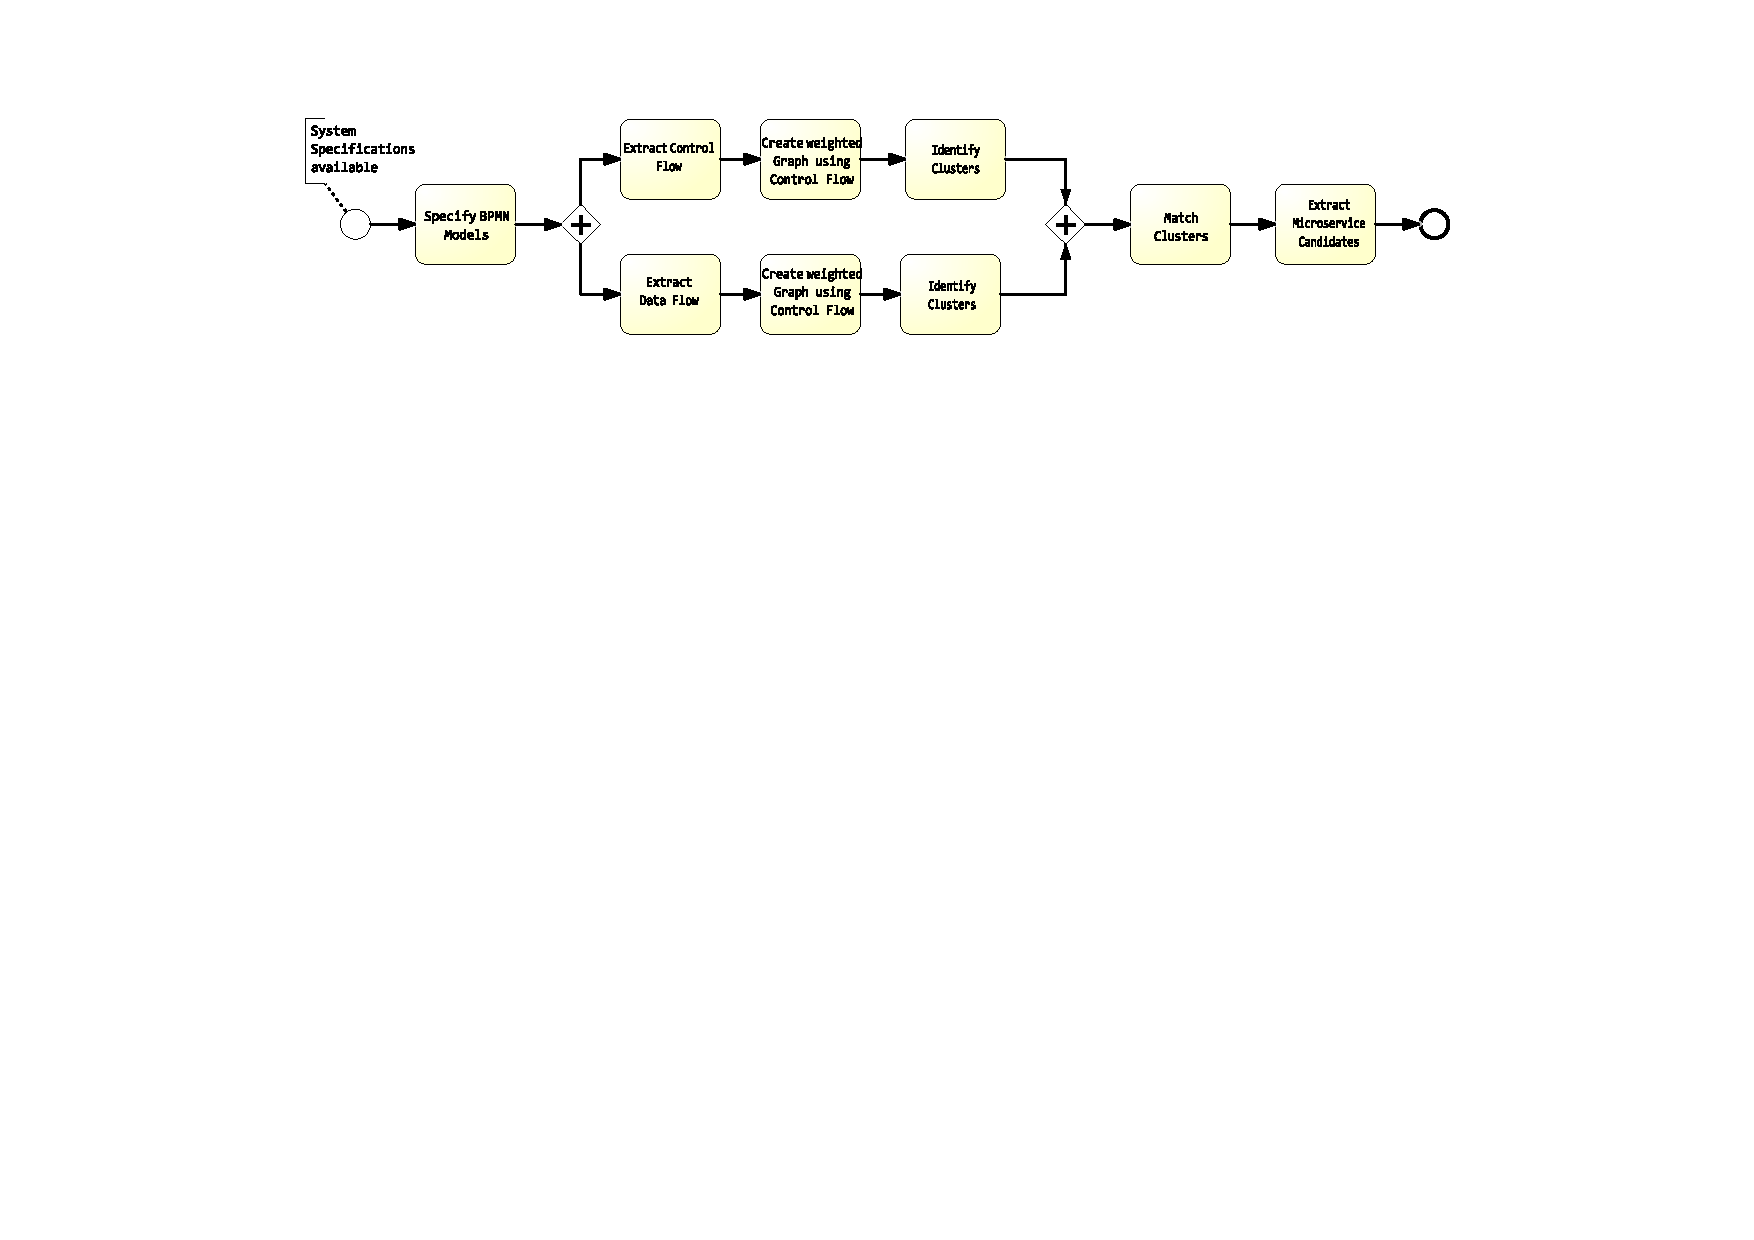
\includegraphics[width=\textwidth, trim={7.5cm 15.3cm 5.0cm 1.5cm}]{img/ThesisProcess.pdf}
	\caption{Overview of the identification approach}
	\label{fig:thesisProcess}
\end{figure}






\section{Specify BPMN Models}
\label{sec:Solution:SpecifyBPMN}
Chapter \ref{ch:PrepApproach}, introduces the BPMN 2.0 modelling language as an easy to use, but yet powerful notation to illustrate business processes including their activities and their data needs.
In the first step of the solution, those business processes need to be specified. Usually, the system specification are not directly given in form of business processes, bur rather in the form of use cases, UML models, domain models or even as textual description in natural language. Therefore, the first step consists of specifying a business model using the available system specification. This can be achieved using various approaches, for instance: \\

\noindent
\textbf{Workshops} At the very beginning of a software project, technical and non-technical stakeholders can participate in a workshop to specify the business process model. As illustrated in the BPMN specification, the "primary goal of BPMN is to provide a notation that is readily understandable by all business users"  \cite{OMG}. Therefore, carrying out a workshop with stakeholders from various departments can produce high quality BPMN models which can be further used as input for the extraction process.\\

\noindent
\textbf{Use Cases} In the case of CoCoME, the system specifications are available as use cases (cf. chapter \ref{ch:CoCoME}). Accordingly, section \ref{sec:PrepApproach:TransformUCtoBPMN} illustrates a process to transform use cases into BPMN models. 
\\

\noindent
\textbf{Others} Business processes can be extracted in various other ways. UML Activity diagrams, for instance, are very similar to BPMN models. Van der Aalst et al. elaborated the Process Mining Manifesto \cite{ProcessMiningManifesto} where he presents general techniques to extract business processes, although it is mainly event log driven. Another approach is the \textit{BPMN Miner}, an automatic discovery tool for BPMN process models \cite{BPMNMiner}. Again, the tool discovers the models dynamically, using log files of a legacy system.



\section{Extract Control Flow}
\label{sec:Solution:ExtractControlFlow}
In the course of the process, activities of the business processes are clustered based on their structural dependency which is extracted from the control flow. Activities (tasks) in business processes play the role of operations in microservices, representing the functionality a service is able to offer. During the process of microservice identification, it is desired to cluster high cohesive functionality into one microservice. To achieve this, one must first extract the structural  dependencies between activities in business processes. \\
The extraction process itself is trivial, as the business process language BPMN was designed to illustrate the control flow between activities (cf. Sec.\ref{sec:PrepApproach:BPMN}). Mainly inspired by the work of M. Amiri in \textit{Object-aware Identification of Microservices} \cite{ObjectAwareAmiri}, we propose a straightforward technique to separate the control flow information from BPMN 2.0 models in section \ref{ch:PrepApproach:ControlDataFlowBPMNProcess}.




\section{Extract Data Flow}
\label{sec:Solution:ExtractDataFlow}
Besides the structural dependencies of activities, data object access plays a significant role in the definition of microservices. As depicted in the background chapter \ref{ch:background}, microservice generally administer their own database with the data entities that belong to the bounded context of the service. Nevertheless, data needs to be shared among services which raises the question where to place a shared data object. Like the previous section, we propose to use clustering based on data flow to identify high cohesive but loosely coupled set of data object clusters. \\
When BPMN 2.0 was introduced, the language was extended by the ability to represent data objects that are consumed and/or produced by the activities. Despite the fact that BPMN is still a language to illustrate the control flow of business processes, the extension provides th possibility to visualize the data flow. In Sec.\ref{ch:PrepApproach:ControlDataFlowBPMNProcess}, we present a formal approach to extract the data flow by discarding anything but flow elements used to represent the data flow.



\section{Create weighted Graph on Control Flow}
\label{sec:Solution:CreateGraphControl}
As depicted in the background chapter \ref{ch:background}, microservices are high cohesive, loosely coupled and fine-grained. 

It is desired to have 

Decomposing business processes into microservices 

BPMN was originally designed to illustrate the control flow between activities. 

Here the problem is to identify appropriate
microservices by decomposing each business process in a way
such that the identified microservices are cohesive, loosely
coupled, and fine-grained. In other words, each activity of a
business process plays the role of an operation (functionality
in one microservice and we want to cluster all the activities
of a business process. Each cluster is then introduced as a
microservice.
To find such microservices, one may take the structural
dependency of activities into account and cluster activities
based on the edges in the process model: if there is a direct
edge between two activities within a business process, those
two activities are more likely two be clustered in the same
microservice. Fig. 2(a) shows the microservices identified from
the PlanApproval process using this approach where the
process decompose into 4 microservices.


\section{Create weighted Graph on Data Flow}
\label{sec:Solution:CreateGraphData}


\section{Identify Cluster}
\label{sec:Solution:IdentifyCluster}

\section{Match Cluster}
\label{sec:Solution:MatchCluster}
Having both sets of clusters...

\section{Extract Microservice Candidates}
\label{sec:Solution:ExtractMicroserviceCandidates}




\section{Distance Metric}
\begin{itemize}
	\item Determine distance between pair of Objects in BPMN (Count activities in between)
	\item Basic Idea: Data accessed more successively is more connected and belongs to same service
	\item Pro: Easy
	\item: Contra: Not really Data Flow; pair  occurs several times --> On time close, other times far away, what about average?
\end{itemize}

\section{Count Activities Metric}
\begin{itemize}
	\item Count activities that access a pair of objects in BPMN
	\item Basic Idea: Data frequently accessed together is more connected and belongs to the same service
	\item Pro: represents idea of data cohesiveness
	\item Contra: Again activities (no clean data flow) but nothing else!

\end{itemize}





